% The methods that you use goes here

Using ParMooN\textsuperscript{[1]}, an in-house FEM package, we solve the time dependent Navier-Stokes equation using variational multi-scale method. And using its results, the particles are simulated by a Lagrangian approach\textsuperscript{[2]}. The equations of motion for the particles are given by

\begin{alignat*}{2}
     m_p\frac{d\mathbf{u}_p}{dt} =& \frac{3}{4}\frac{\rho_f}{\rho_p}\frac{m_p}{d_p}\frac{C_D}{C_C}\left|\mathbf{u}_f - \mathbf{u}_p\right|\left(\mathbf{u}_f - \mathbf{u}_p\right)  \\
     &+ m_p\mathbf{g}\frac{\rho_p - \rho_f}{\rho_p} + \mathbf{F}_B
\end{alignat*}

Here $\mathbf{u}_p$, $\mathbf{u}_f$, $\rho_p$, $\rho_f$,  represents the particle velocity, fluid velocity, particle density and fluid density respectively. The terms in the right hand side are drag force, gravitational force and Brownian force respectively.

\begin{itemize}
\item The above equation is used to update the particle's current position at every time-step
\item Based on the current position, the current cell is determined using a zonal-based search
\item If the particle is outside the domain, based on the previous cell and current position, the deposition location is computed
\end{itemize}

\vspace{0.3cm}
\begin{center}
  \vspace{-0.4cm}
  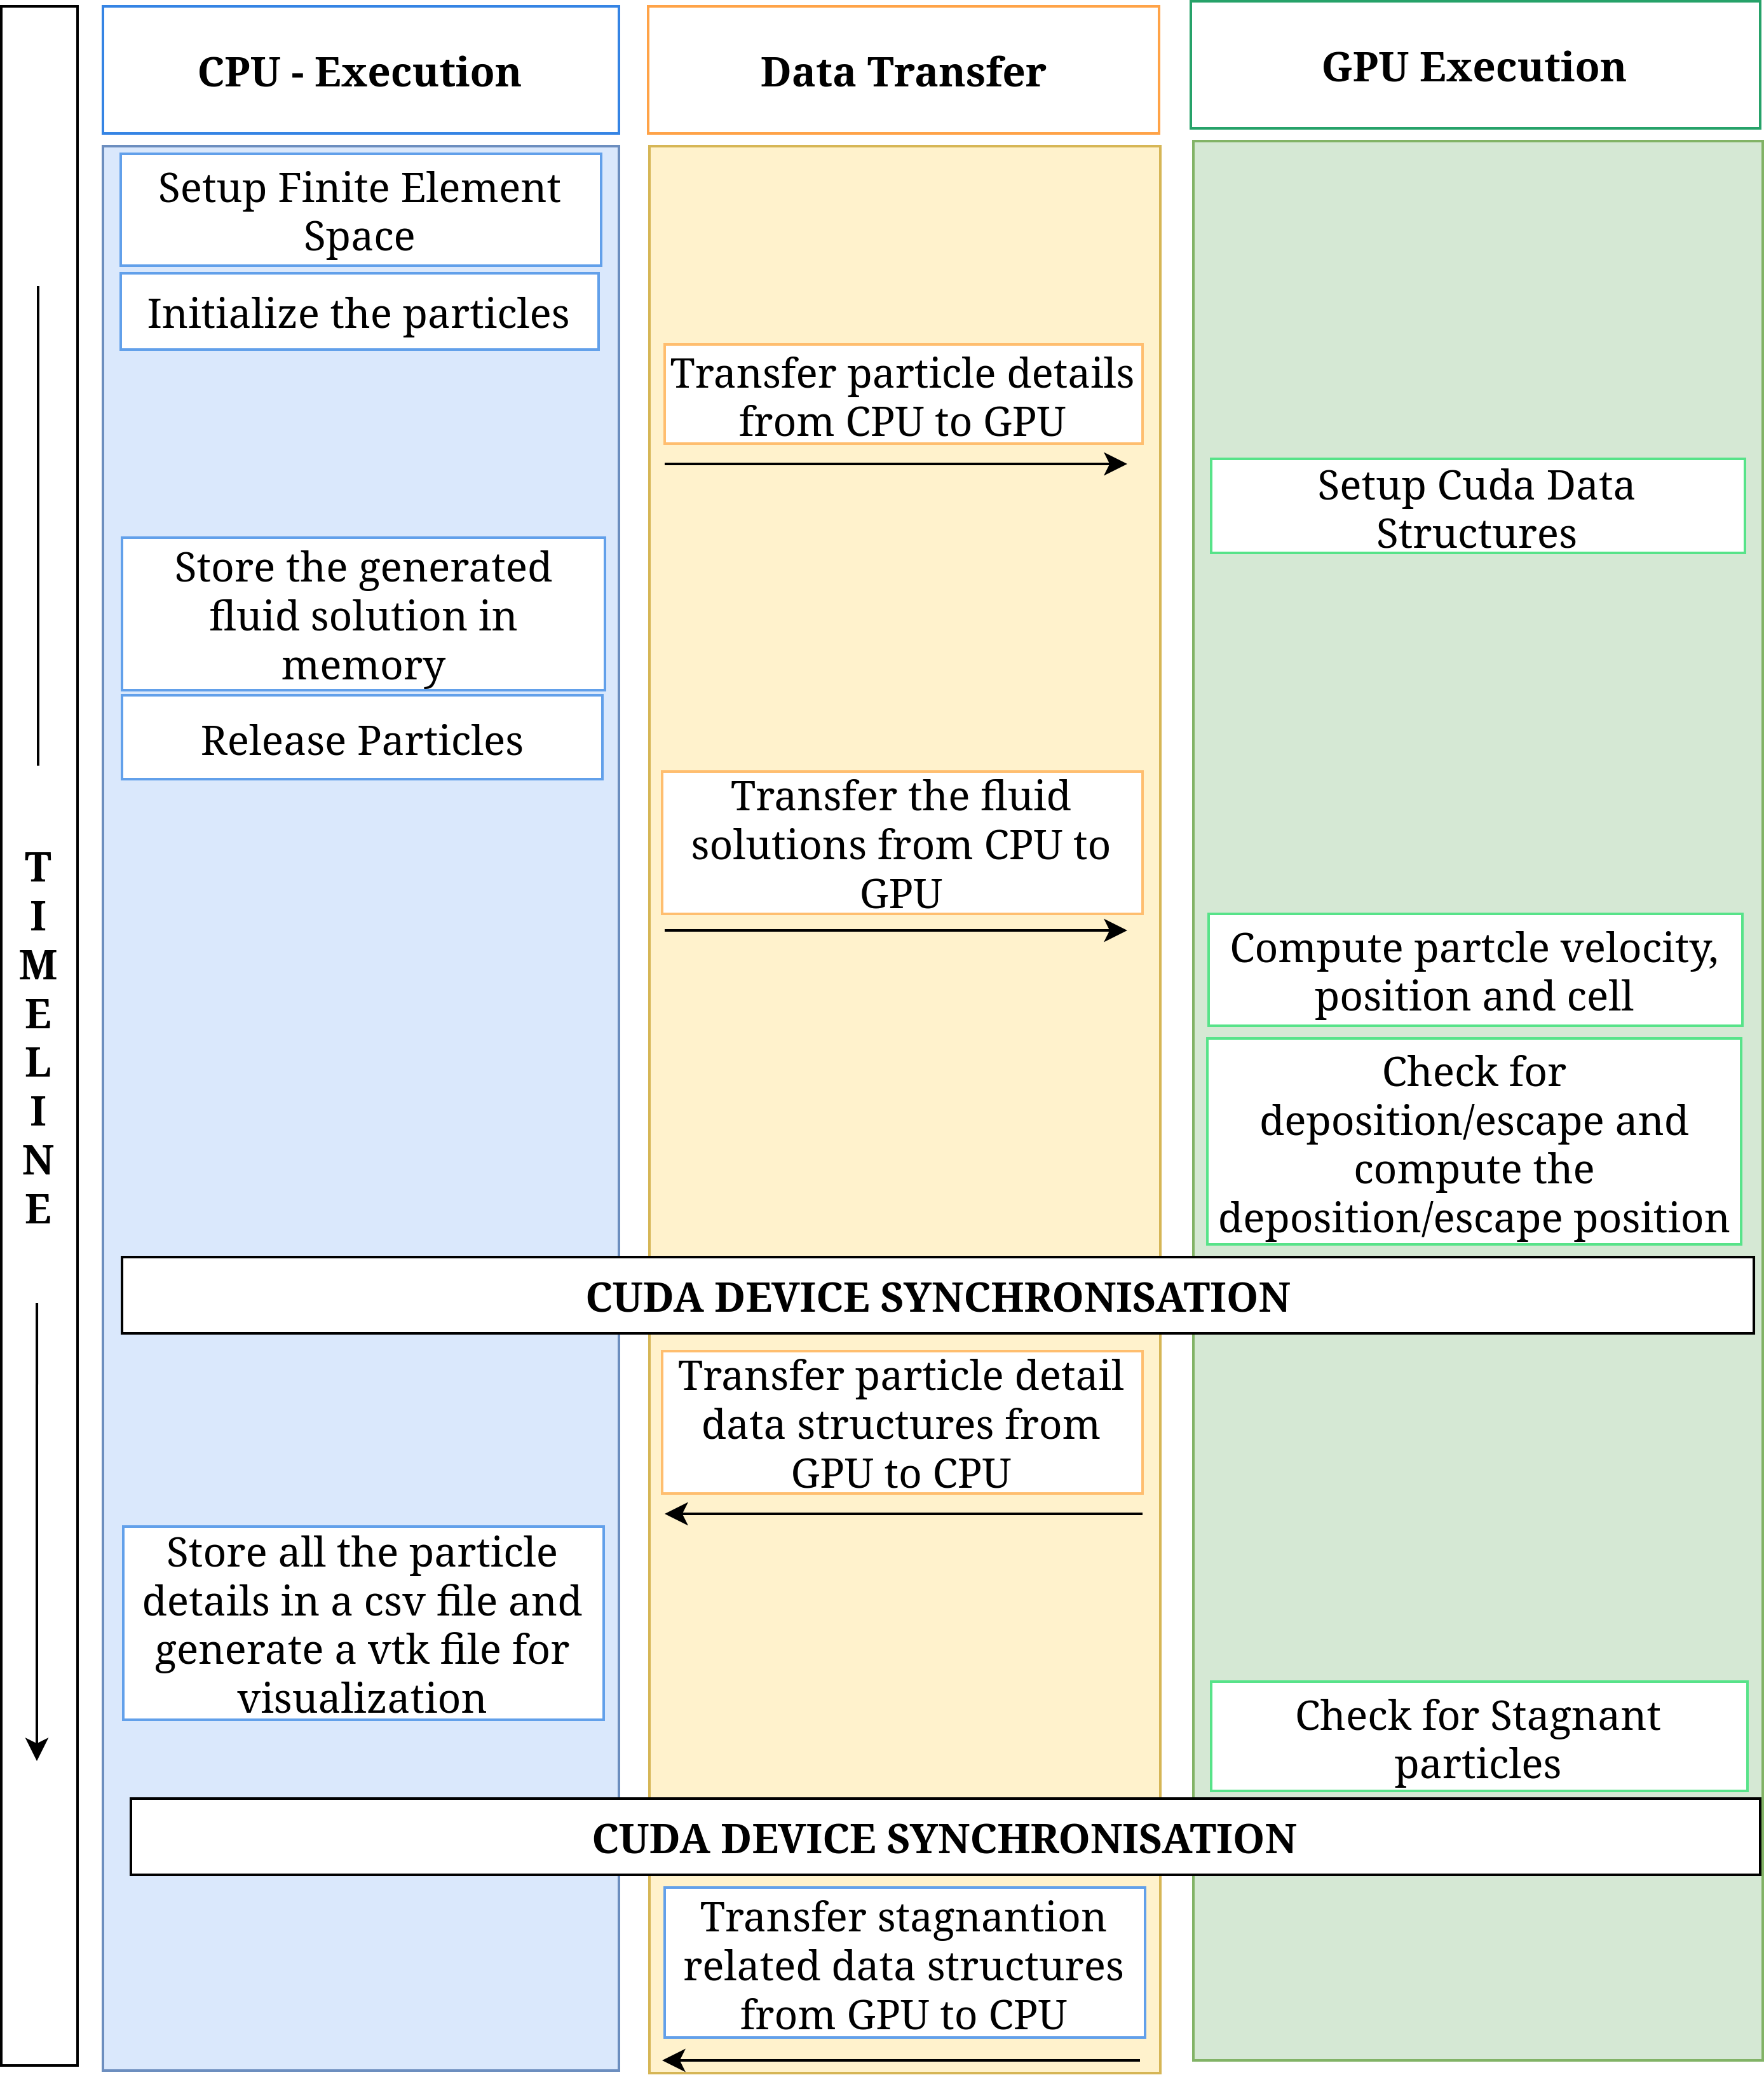
\includegraphics[width=.5\linewidth]{timeline}
\end{center}

\begin{itemize}
\item Mesh, Geometry (segmented), Begining of simulation, End of simulation
\end{itemize}
\vspace{0.1cm}
\begin{center}
  \vspace{-0.4cm}
  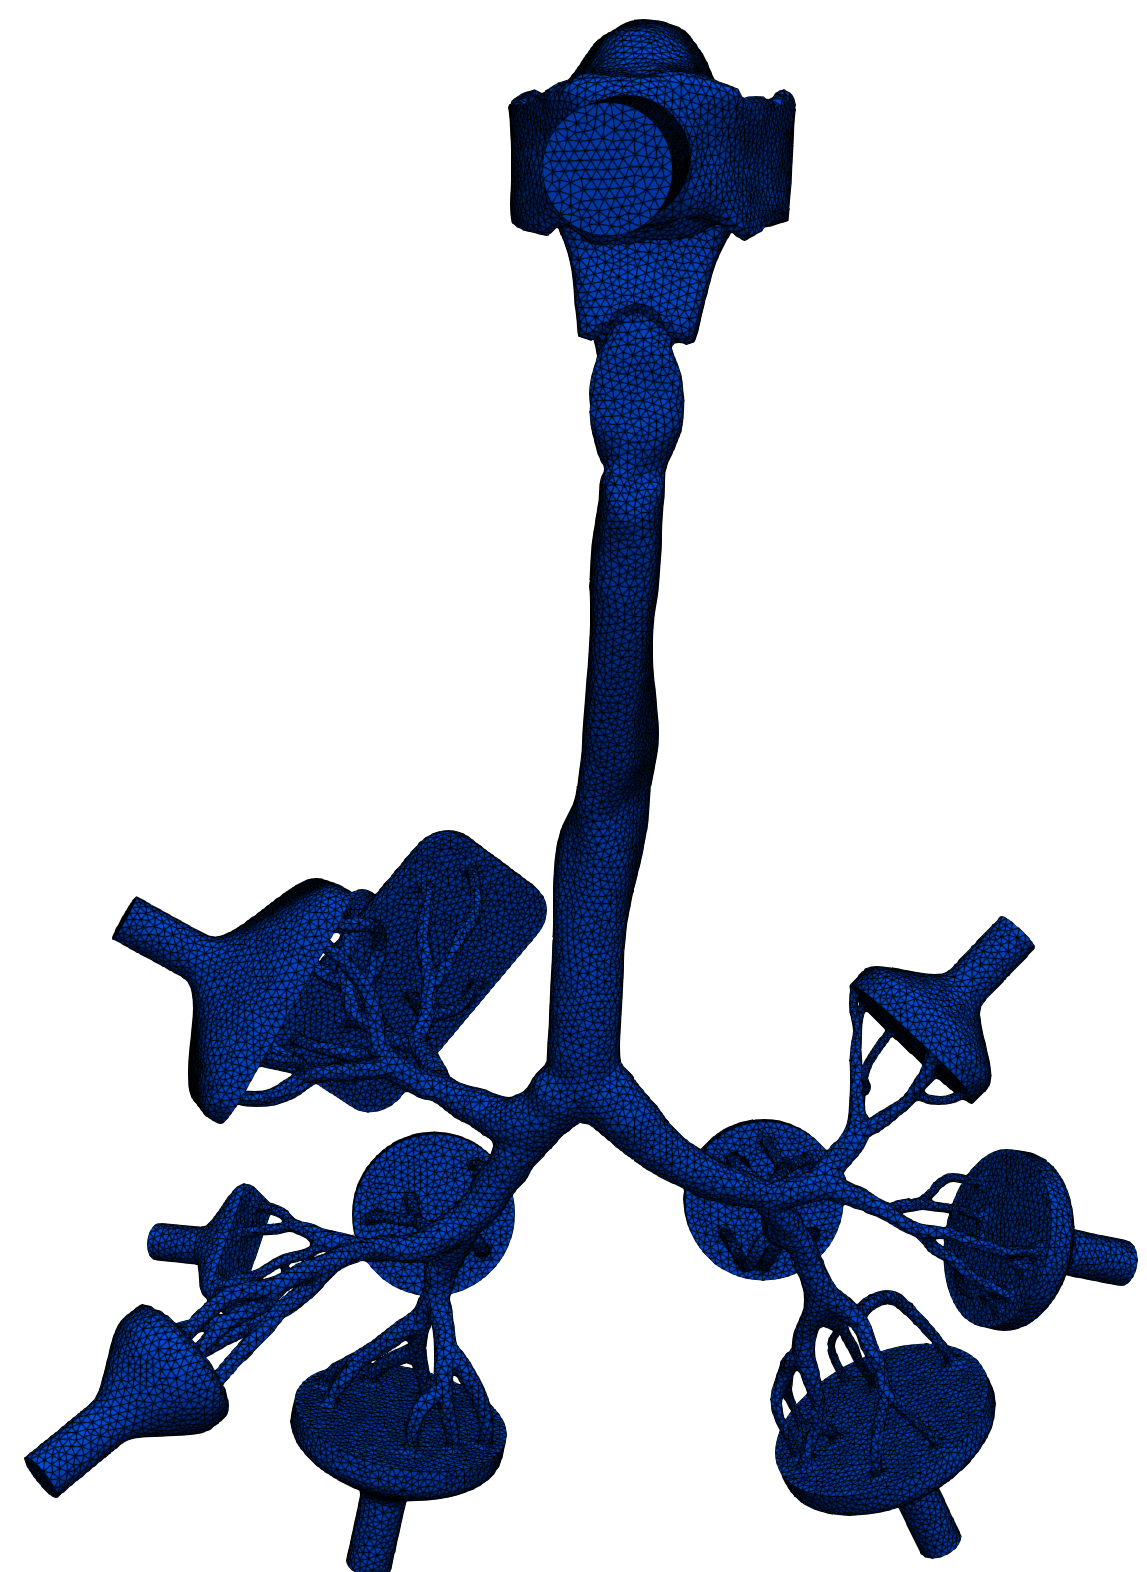
\includegraphics[width=.2\linewidth]{mesh}%
  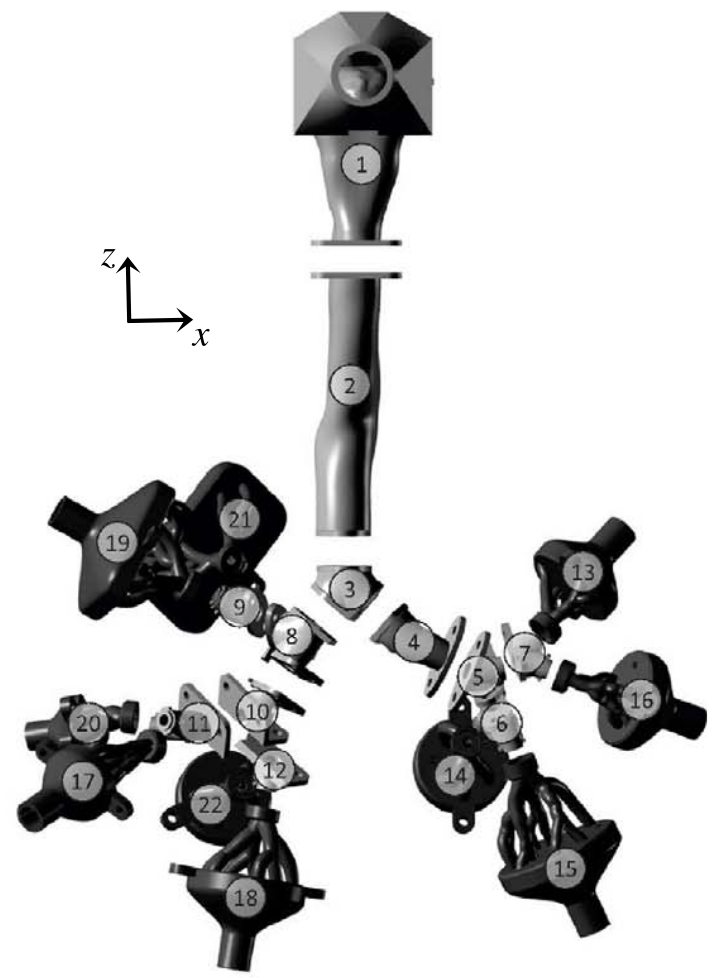
\includegraphics[width=.2\linewidth]{segments}\hspace{0.2cm}
  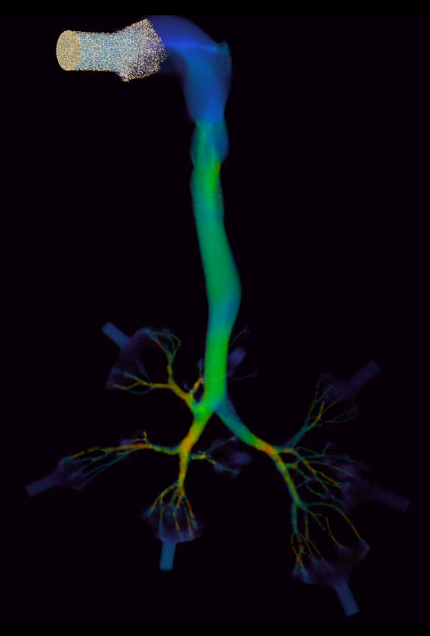
\includegraphics[width=.2\linewidth]{simulation_beg}%
  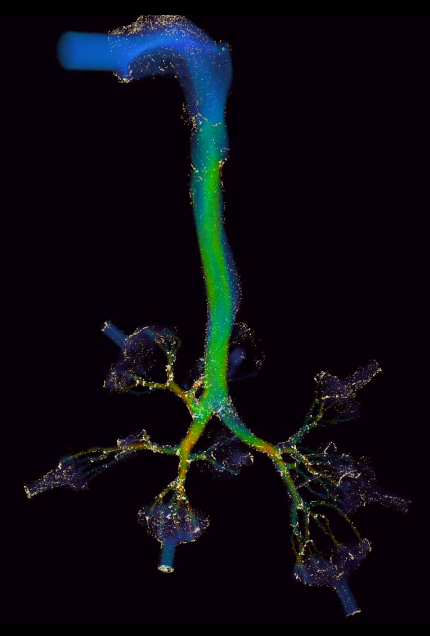
\includegraphics[width=.2\linewidth]{simulation_end}
\end{center}
% \vspace{0.25em}

% \vspace{0.3cm}
% \begin{center}
%   \vspace{-0.4cm}
%   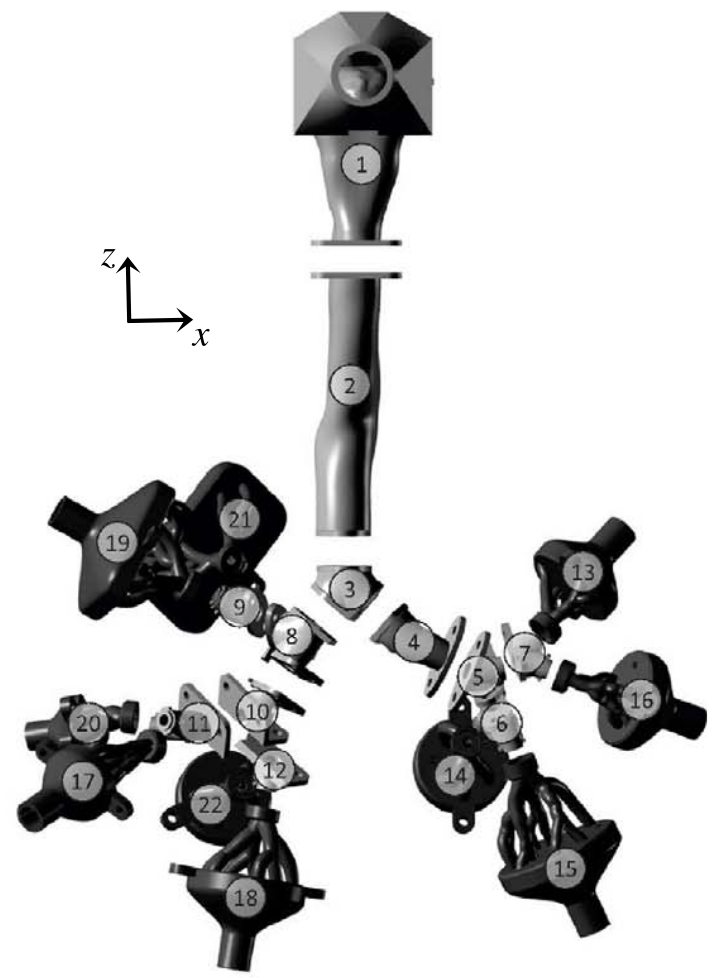
\includegraphics[width=.4\linewidth]{segments}%
%   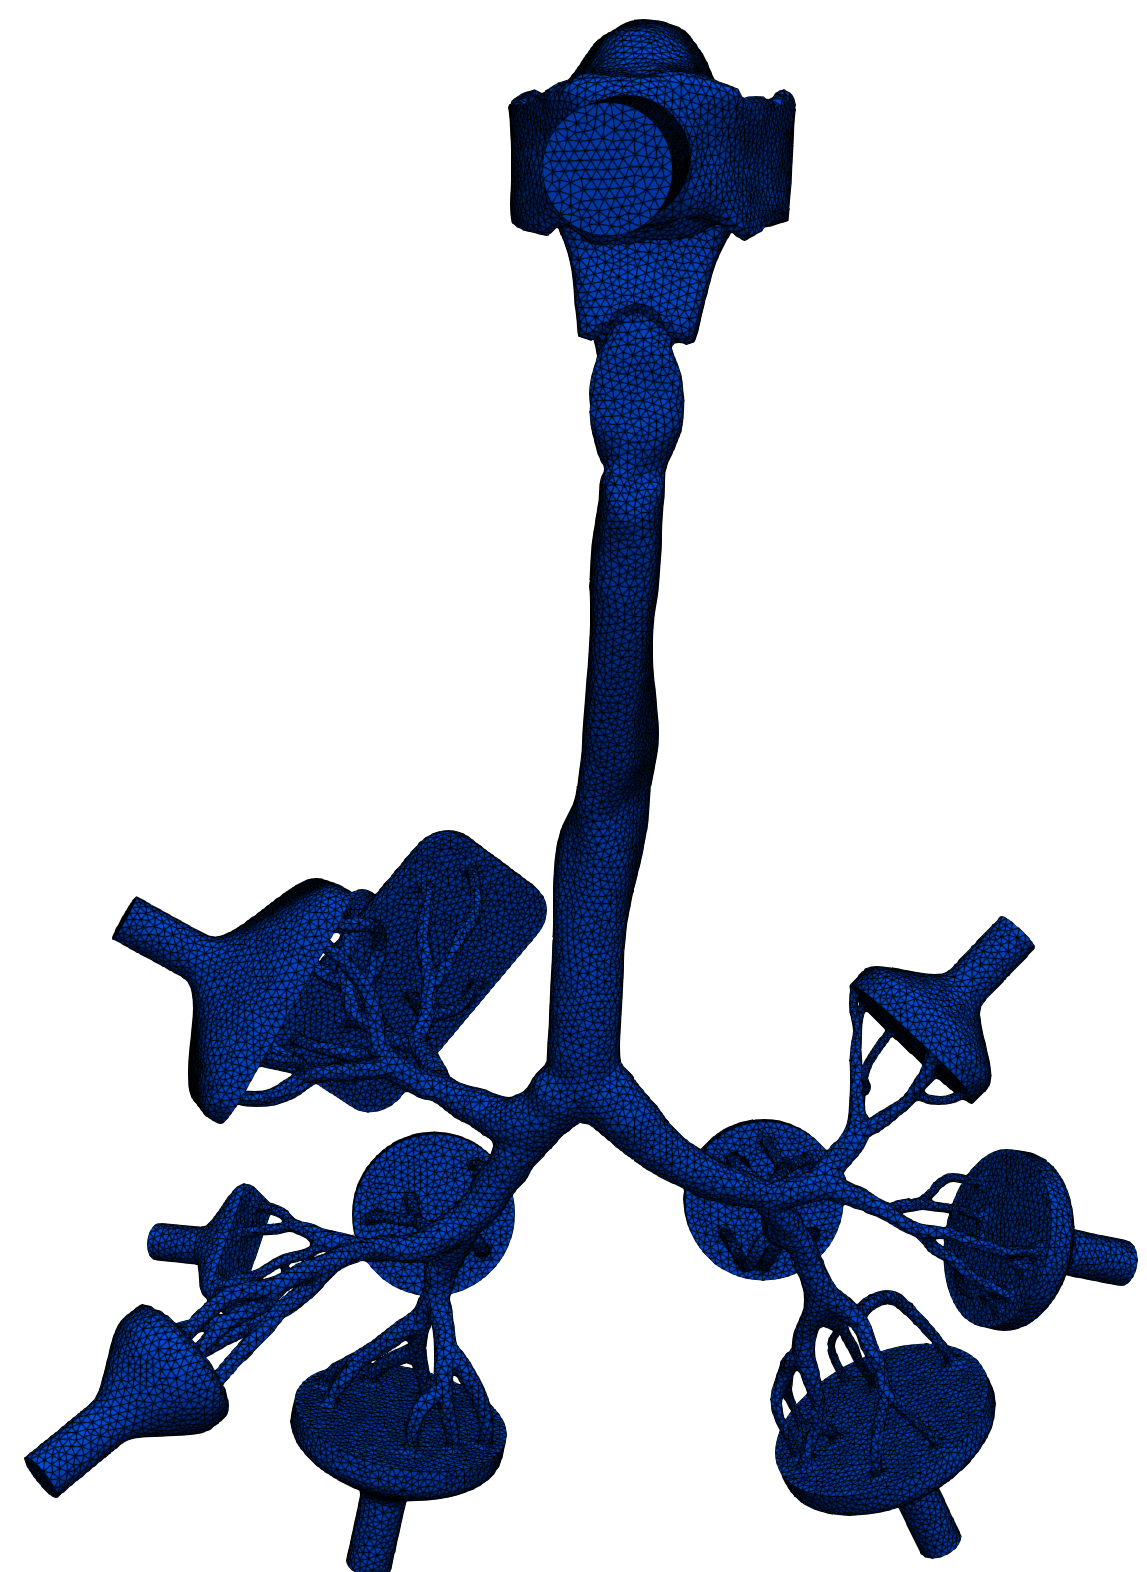
\includegraphics[width=.4\linewidth]{mesh}
% \end{center}
% \vspace{0.25em}
% \textbf{Computational Mesh:}

% \begin{tabular}{@{$\bullet$ }ll}
% Number of Vertices  &: 65,725 \\
% Number of Cells     &: 276,577   \\
% Number of Boundary faces &: 590,950 \\
% DOF velocity fluid: &: 1,337,640 \\
% DOF velocity pressure &: 65,725 \\
% \end{tabular}

\vspace{2em} % Fill in to put references at the bottom